\newpage
\section{Data Extraction}
\label{sec:algorithm}
First step that program supposed to do is to load data and to compute connected components. Data is stored in GML file format. More detail information about this format and other common graph file formats is given in Section~\ref{sec:algorithm}.

\subsection{Dataset Description}
\label{sec:dataset_description}
Gene Ontology data and cluster analysis results presented as directed graphs. They are stored in separate files in special format --- GML files.


GO graph is directed acyclic graph that has 10,042 vertices and  24,155 edges. Also it has 1 root, 2,729 nodes and 7,312 leafs (terminal nodes).
Figure~\ref{fig:yed_GO_vis} shows visualization of the Gene Ontology graph using Hierarchical layout by yEd~\cite{yed} graph editing tool. It obviously shows imperfectness of classic visualization of graphs.


\begin{figure}[h!]
\centering
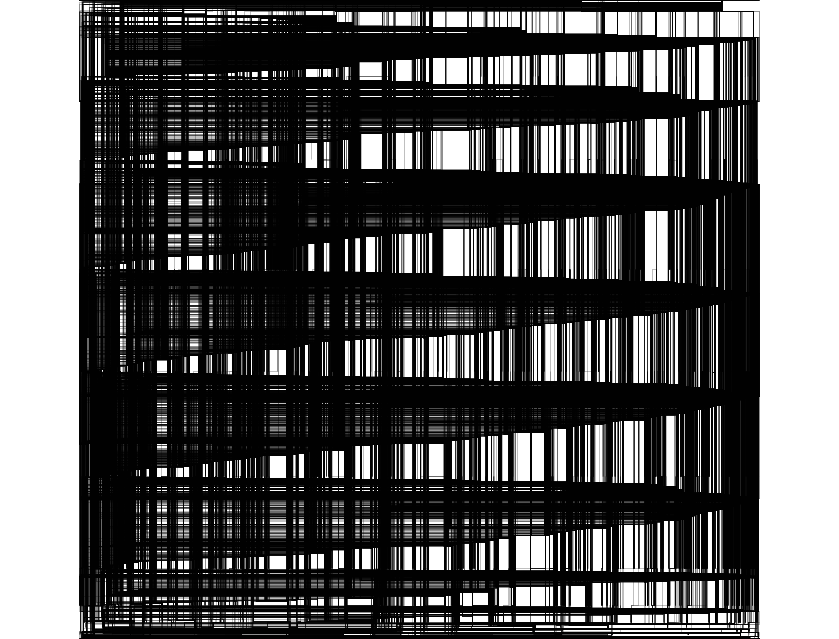
\includegraphics[scale=0.3]{pictures/yEd_GO.png}
\caption{Gene Ontology yEd visualization}
\label{fig:yed_GO_vis}
\end{figure}


Cluster tree is a directed binary graph that has 14,623 nodes and 14,622 edges. The Cluster graph as a tree has a single root, 7,310 nodes and 7,312 leafs.
To get an impression of the graph, Figure~\ref{fig:Cytoscape_Cluster_1} shows the cluster tree that uses the Cytoscape~\cite{Cytoscape} visualization tool.

\begin{figure}[h!]
\centering
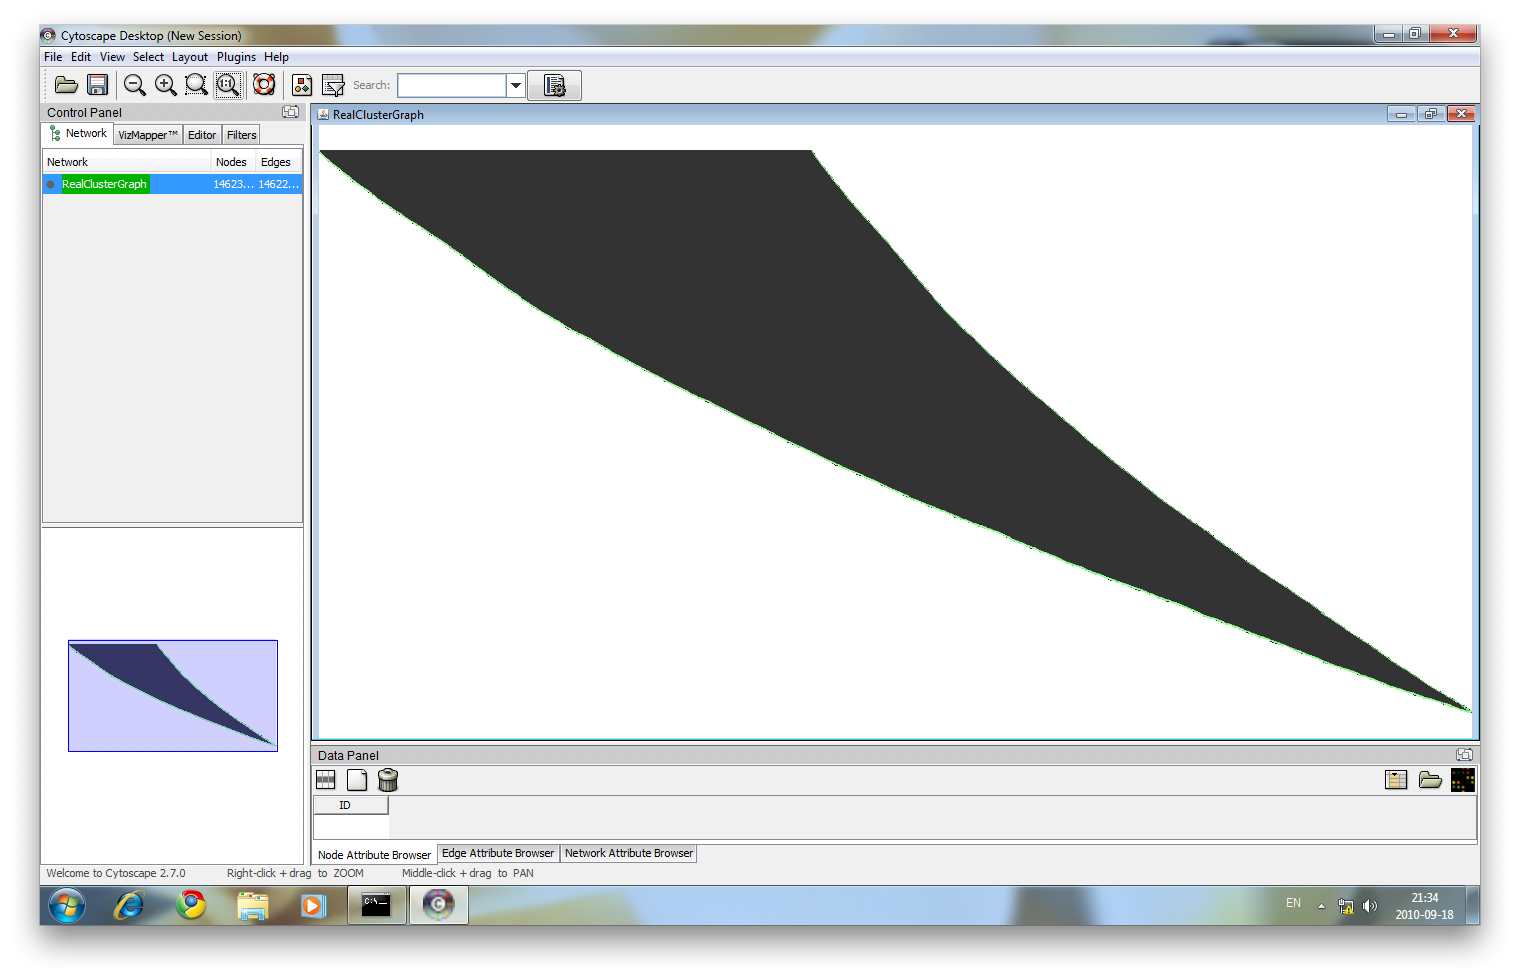
\includegraphics[scale=0.25]{pictures/Cytoscape_cluster_graph_1.png}
\caption{Cluster analysis result tree Cytoscape visualization tool}
\label{fig:Cytoscape_Cluster_1}
\end{figure}

\begin{figure}[h!]
\centering
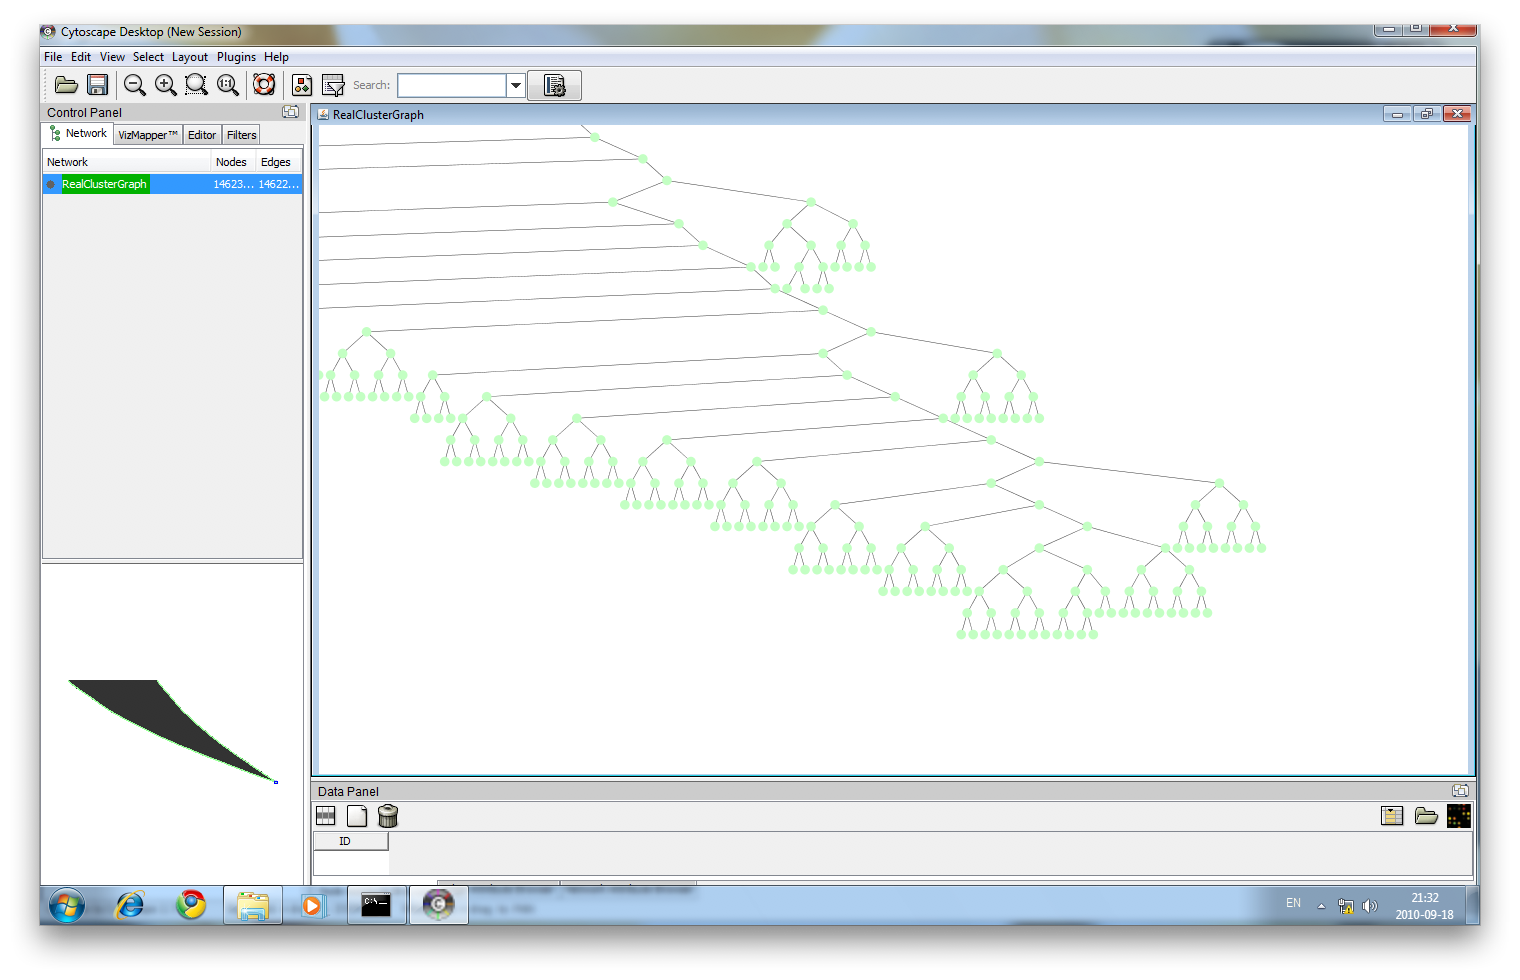
\includegraphics[scale=0.25]{pictures/Cytoscape_cluster_graph_2.png}
\caption{Zoomed cluster analysis result tree}
\label{fig:Cytoscape_Cluster_2}
\end{figure}

Both graphs are independent from each other based on developer point of view: they have different node ids and edge ids. More over, they are connected by vertex labels ---
both graphs have same labels for terminal (leaf) vertices. This property is used in the sub-graph extracting algorithm.


Performance is one of the main requirements since the application should work with large quantity of data that has over tens of thousands vertices. It is very important to give a consideration on optimization.


\subsection{Mapping Algorithm}
\label{sec:mapping_algorithm}
Here is the explanation of that program algorithm uses sample graphs:
\begin{enumerate}

\item The program visualizes Gene Ontology and cluster analysis result tree. This visualization technique is discussed in Section~\ref{sec:solution}.

\begin{figure}[h!]
\centering
\subfloat[Selected node in the Gene Ontology]{
    \label{fig:step_1}
    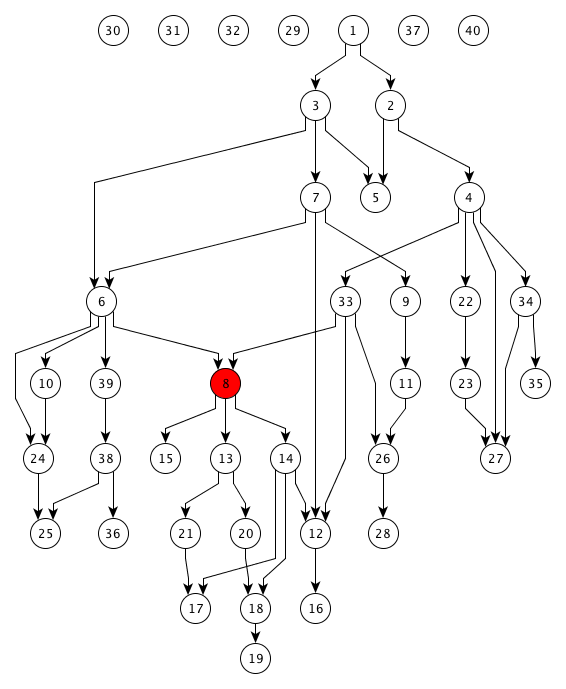
\includegraphics[scale=0.3]{pictures/subgraph_extraction_algorithm_step_1.png}
}
\subfloat[Extract sub-graph for selected node]{
    \label{fig:step_2}
    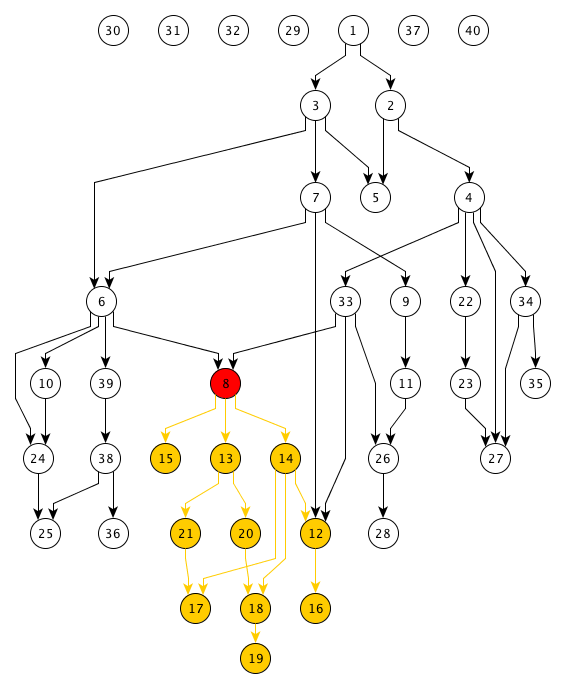
\includegraphics[scale=0.3]{pictures/subgraph_extraction_algorithm_step_2.png}
}
\caption{Sub-graph extraction from the Gene Ontology}
\end{figure}

\item Interactively select node in the Gene Ontology graph (Figure~\ref{fig:step_1}).

\item When node is selected the program computes all successors (Figure~\ref{fig:step_2}).

\item Extract leafs from successors (Figure~\ref{fig:step_3}).

\begin{figure}[h!]
\centering
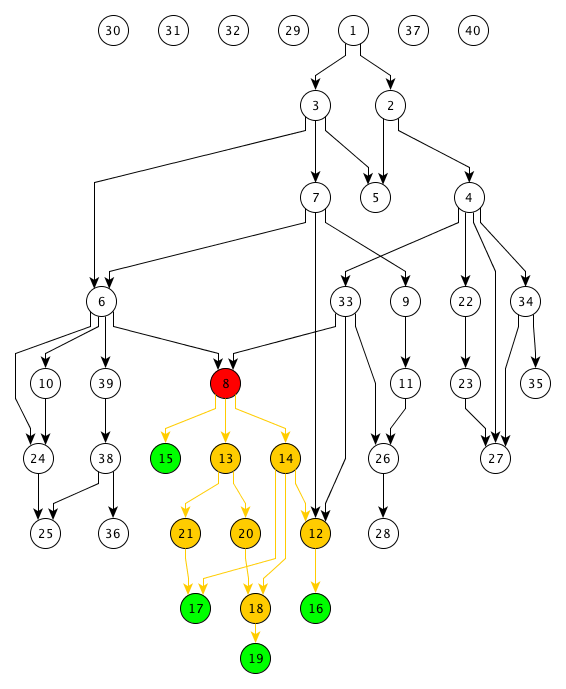
\includegraphics[scale=0.5]{pictures/subgraph_extraction_algorithm_step_3.png}
\caption{Extract leafs from the Gene Ontology sub-graph}
\label{fig:step_3}
\end{figure}

\item On this step program finds sub tree and caches. This sub tree is highlighted in cluster analysis tree.

\item The program searches corresponded leaves in cluster analysis result tree by label, as showed in Figure~\ref{fig:step_4}.

\item For any item the program finds root connected to all leaves and extracts corresponding sub trees (Figure~\ref{fig:step_5}).
\end{enumerate}

\begin{figure}[h!]
\centering
\subfloat[Find corresponded leafs]{
    \label{fig:step_4}
    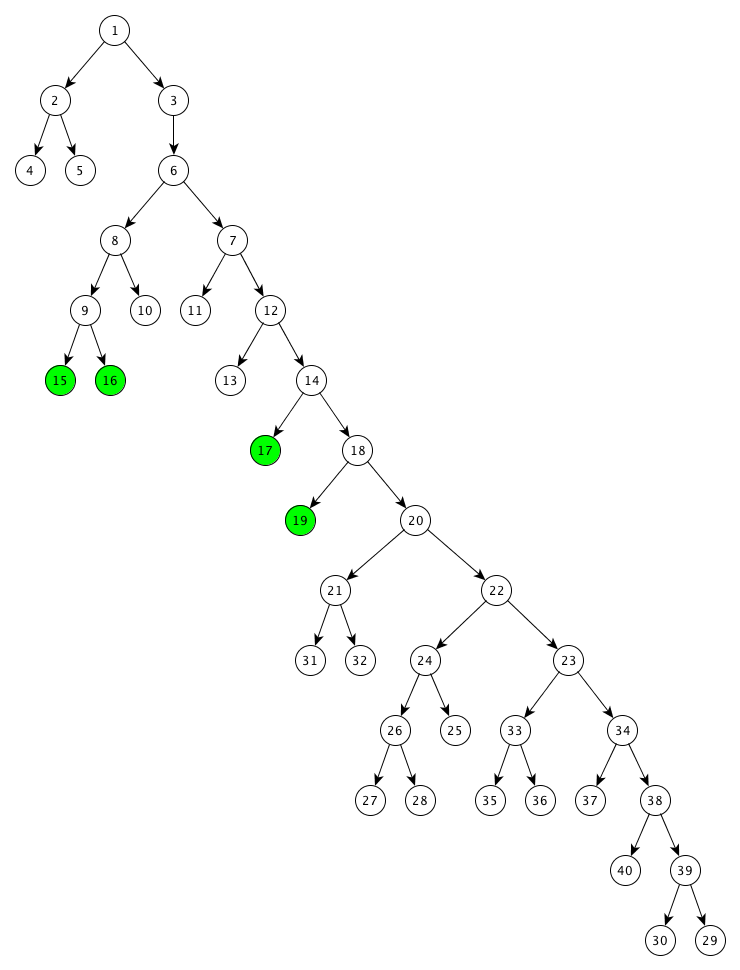
\includegraphics[scale=0.23]{pictures/subgraph_extraction_algorithm_step_4.png}
}
\subfloat[Build sub-graph]{
    \label{fig:step_5}
    
    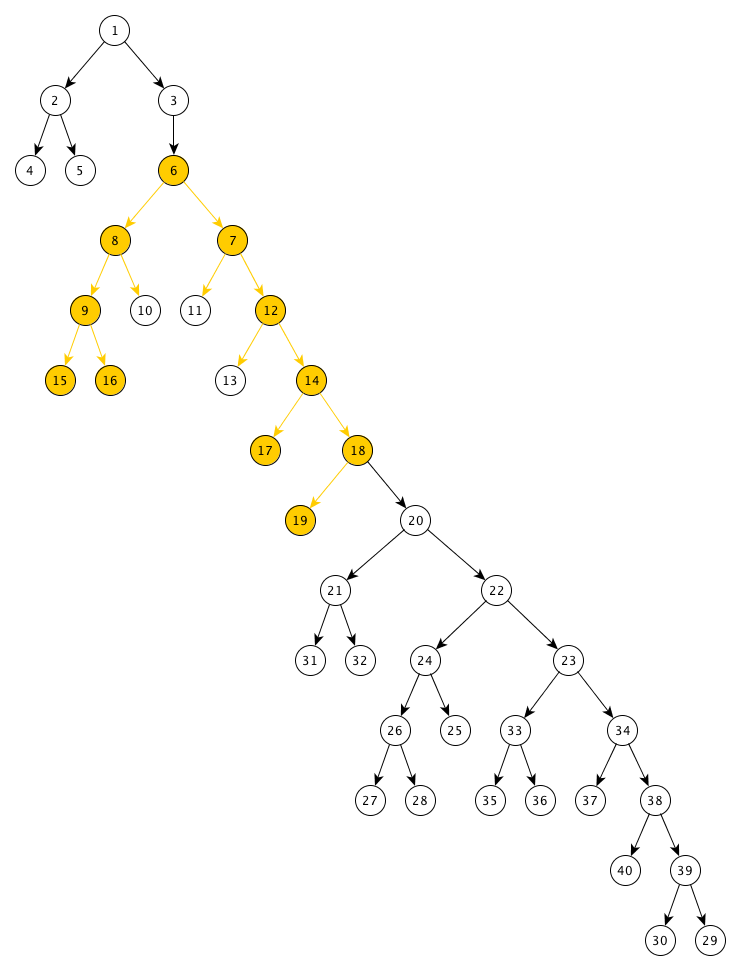
\includegraphics[scale=0.23]{pictures/subgraph_extraction_algorithm_step_5.png}
}
\caption{Analyze Cluster graph}
\end{figure}


As was mentioned before, the aim of the work is to provide flexible tool specially made for biology scientists to deal with huge data sets.
To trace relations in the two separated datasets (Gene Ontology graph and cluster analysis result tree): both graphs are stored separately in the different files.
Also during program design we had to consider that cluster analysis results graph was produced from Gene Ontology graph using separate tool and clustering algorithm specific to the purpose.
This means that there are various cluster graphs for the same Gene Ontology.

The tools provides effective space filling visualization method and allows interactive relations highlighting.
The tool also provides ability to track graphs discovering: focused or selected vertex and label are showed for both graphs separately.

Considering end-user requirements there is a use case specification for biology scientist ---
interest in the concrete gene in the Gene Ontology. Also scientists are interested in the search mechanism to find specific gene by name and view it immediately on the graph.